\documentclass[tikz, border=2mm]{standalone}
\usepackage{amsmath}
\usetikzlibrary{automata, positioning, arrows}
\tikzset{
  ->, % makes the edges directed
  >=stealth', % makes the arrow heads bold
  node distance=3cm, % specifies the minimum distance between two nodes. Change if necessary.
  every state/.style={thick}, % sets the properties for each ’state’ node
  initial text=, % sets the text that appears on the start arrow
}

\begin{document}

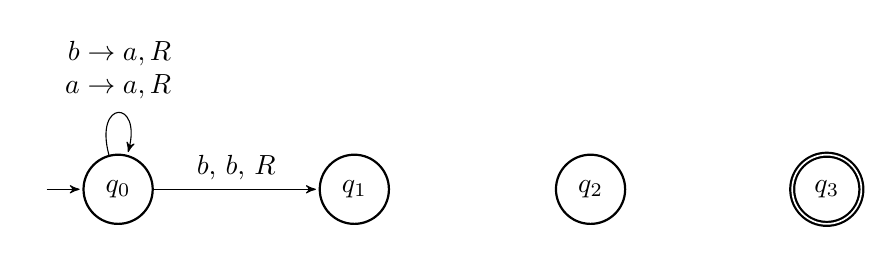
\begin{tikzpicture}[shorten >=1pt, on grid, auto]
  \node[state, initial] (1) {$q_0$};
  \node[state, right of=1] (2) {$q_1$};
  \node[state, right of=2] (3) {$q_2$};
  \node[state, right of=3, accepting] (4) {$q_3$};

  \draw (1) edge[above] node{$b$, $b$, $R$} (2)
        (1) edge[loop above] node[above]{$
    \begin{aligned}
      b &\to a, R\\[-0.7ex]
      a &\to a, R
    \end{aligned}$} (1);
    
\end{tikzpicture}

\end{document}